\scanpage{182}

\margin{$g,\nu$}

$X$ \uline{propre}

1°) Connexe, lisse \inserted{\unsure{sauf}} pts doubles ordinaires
\inserted{(diviseur $D$)}, dim $1$

2°) $\chi(\deleted{\unsure{X,}}\underline{\mathcal O}_X)\deleted{\unsure{g}}=1-g$

i.e. si $\widetilde X^{\unsure{*|+}}$ la \unsure{normalisée}, $g_i$ les genres,
$\mu$ le nb des pts doubles
\[
g-1=\sum(g_i-1)+\mu
\]
\[
g=\sum g_i+\mu+1-s
\]

\margin{$s$ nb de comp. irr.\\
$\mu$ \rule{1.8cm}{.4pt} pts doubles\\
(\uline{NB} on a tjrs $\mu+1-s\geq0$\\
à cause connexité)}

\margin{
\figure{
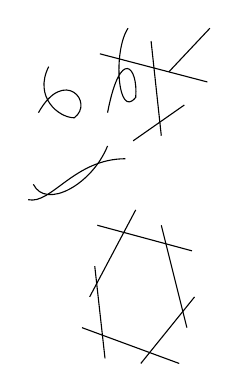
\begin{tikzpicture}[x=.65cm,y=.65cm]
\draw (.1,3.8) .. controls (-.2,3.2) and (.3,2.8) .. (.6,2.8)
 .. controls (1,3.1) and (.4,3.8) .. (-.1,2.9);
\draw (1.25,2.9) .. controls (1.5,4.2) and (1.85,3.8) .. (1.8,3.2)
 .. controls (1.45,2.75) and (1.35,4.1) .. (1.65,4.55);
\draw (1.1,4.05) -- (3.2,3.5);
\draw (2.1,4.3) -- (2.3,2.45);
\draw (2.45,3.7) -- (3.25,4.55);
\draw (1.75,2.35) -- (2.75,3.05);
\draw (-.2,1.5) .. controls (.05,1) and (.95,1.5) .. (1.25,2.25);
\draw (-.3,1.2) .. controls (.15,1.1) and (.6,2.0) .. (1.6,2.0);
\draw (1.05,.7) -- (2.9,.2);
\draw (1.8,1) -- (.9,-.7);
\draw (1,-.1) -- (1.2,-1.9);
\draw (.75,-1.3) -- (2.65,-2.0);
\draw (1.9,-2.0) -- (2.95,-.7);
\draw (2.3,.7) -- (2.8,-1.3);
\end{tikzpicture}
}}

3°) $S\subset X$ \deleted{\unsure{fini|un}} \deleted{\unsure{multisecti.} étale diviseur}
\inserted{sous-schéma. fini étale, de rang $\nu$}
contenu dans l'\unsure{ouv.} des pts de lissité de $X$

4°) Si $X_i$ comp. irréd. \deleted{de genre} \inserted{avec}
$\widetilde X_i$ genre $1$, alors $X_i$ contient un
pt double \uline{ou} \deleted{\unsure{un}} $X_i\cap S\neq\varnothing$
i.e. $X_i\cap(D\cup S)\neq\varnothing$
($\Longleftrightarrow$ \unsure{Exclu ici.}
pour $X$ lisse de genre $1$, $S=\varnothing$)

5°) Si $X_i$ comp. irréd. avec $\widetilde X_i$ de
genre $0$, alors l'image inverse de $(D\cup S)$ dans
$\widetilde X_i$ a au moins trois pts.

\margin{\figure{\begin{tikzpicture}\draw (.2,0) .. controls (-.1,.1) and (0,1) .. (-.1,1.5) .. controls (-.3,1.7) and (-.1,1.75) .. (-.1,2) -- (-.1,3.2);\end{tikzpicture}}\unsure{pas d'autom. inf. de la} ``situation''}

\figure{\begin{tikzpicture}\draw (0,0) -- (15,1.2);\end{tikzpicture}}

\diagram{
\begin{tikzcd}[column sep=small,row sep=small]
\widetilde D\arrow[r,phantom,"\subset"]\arrow[ddr,"\mathrm{surj}"']&
\underbrace{\widetilde D\amalg S}\arrow[r,"\mathrm{surj}"]\arrow[d,phantom,"\unsure{\wr}"]&
\pi_0(\widetilde X)\arrow[r,"\uline{g}"]\arrow[d,equal]&\mathbb N\\
&\widetilde\Delta&\Delta&\\
&D&&
\end{tikzcd}
}

\margin{$\widetilde D\longrightarrow D$ fibres de $\operatorname{card}\leq2$}

\diagram{
\begin{array}{l}
\left\{
\begin{array}{l}
\operatorname{card}S=\textcircled{$\nu$}\\[2pt]
\displaystyle\sum_{\delta\in\Delta}(g_\delta-1)
+\underbrace{\mu}_{\operatorname{card}\widetilde D}
=\textcircled{$g$}\unsure{+|-}1\\[4pt]
\operatorname{card}\bigl(\unsure{\widetilde D|D}\amalg_{\widetilde D}\Delta\bigr)=1\\
\deleted{\text{fibres de }\widetilde D\longrightarrow\Delta
\text{ de }\operatorname{card}\leq2}
\end{array}\right.
\end{array}
}

\margin{182}
